\chapter{Recurrent neural networks}


\section{Architectures}


\subsection{(Elman) recurrent neural network}

\begin{description}
    \item[Recurrent neural network (RNN)] \marginnote{Recurrent neural network (RNN)}
        Neural network that processes a sequential input. At each iteration, an input is fed to the network and the hidden activation is computed considering both the input and the hidden activation of the last iteration.

        \begin{figure}[H]
            \centering
            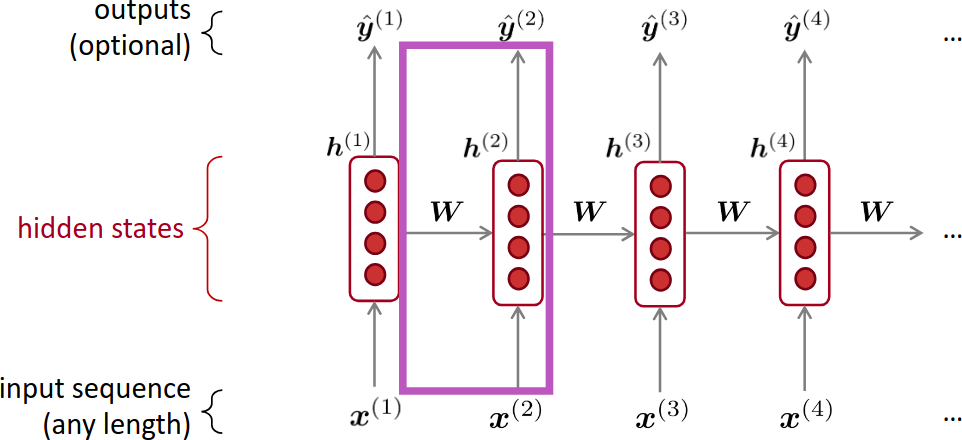
\includegraphics[width=0.5\linewidth]{./img/rnn_unrolled.png}
            \caption{RNN unrolled in time}
        \end{figure}

    \item[RNN language model (RNN-LM)] \marginnote{RNN language model (RNN-LM)}
    Given an input word $w^{(t)}$, an RNN-LM does the following:
    \begin{enumerate}
        \item Compute the embedding $\vec{e}^{(t)}$ of $w^{(t)}$.
        \item Compute the hidden state $\vec{h}^{(t)}$ considering the hidden state $\vec{h}^{(t-1)}$ of the previous step:
        \[ \vec{h}^{(t)} = f(\matr{W}_e \vec{e}^{(t)} + \matr{W}_h \vec{h}^{(t-1)} + b_1) \]
        \item Compute the output vocabulary distribution $\hat{\vec{y}}^{(t)}$:
        \[ \hat{\vec{y}}^{(t)} = \texttt{softmax}(\matr{U}\vec{h}^{(t)} + b_2) \]
        \item Repeat for the next token.
    \end{enumerate}

    \begin{figure}[H]
        \centering
        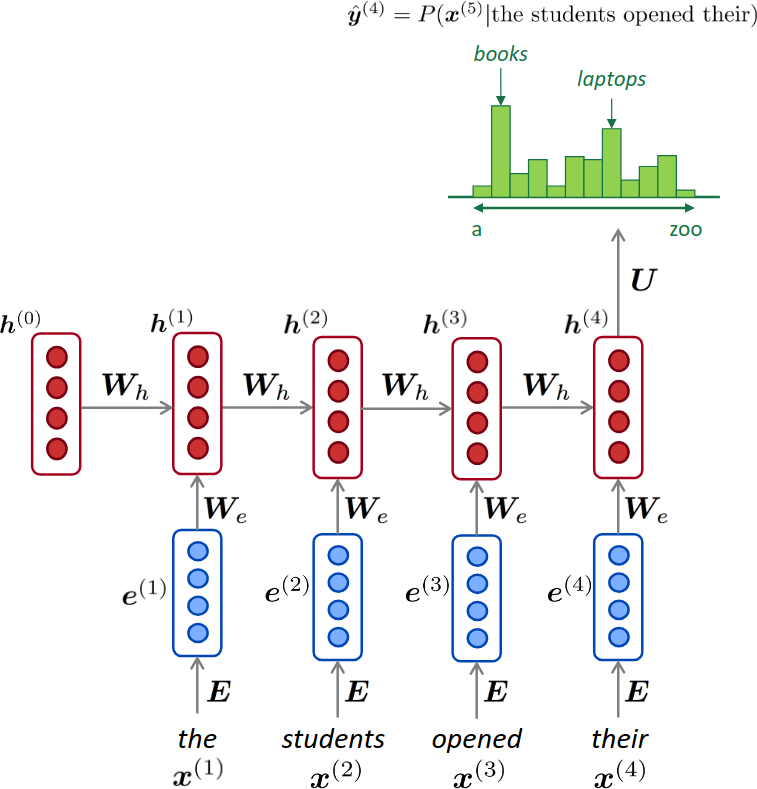
\includegraphics[width=0.4\linewidth]{./img/rnn_lm.png}
    \end{figure}

    \begin{remark}
        RNN-LMs generate the output autoregressively.
    \end{remark}

    \begin{description}
        \item[Training]
            Given the predicted distribution $\hat{\vec{y}}^{(t)}$ and ground-truth $\vec{y}^{(t)}$ at step $t$, the loss is computed as the cross-entropy:
            \[ \mathcal{L}^{(t)}(\matr{\theta}) = - \sum_{v \in V} \vec{y}_v^{(t)} \log\left( \hat{\vec{y}}_v^{(t)} \right) \]

            \begin{description}
                \item[Teacher forcing] \marginnote{Teacher forcing}
                    During training, as the ground-truth is known, the input at each step is the correct token even if the previous step outputted the wrong value.

                    \begin{remark}
                        This allows to stay close to the ground-truth and avoid completely wrong training steps.
                    \end{remark}
            \end{description}
    \end{description}
\end{description}



\section{Applications}

\subsection{Autoregressive generation}

\begin{description}
    \item[Autoregressive generation] \marginnote{Autoregressive generation}
        Repeatedly sample a token and feed it back to the network.

    \item[Decoding strategy] \marginnote{Decoding strategy}
        Method to select the output token from the output distribution. Possible approaches are:
        \begin{descriptionlist}
            \item[Greedy] Select the token with the highest probability.
            \item[Sampling] Randomly sample the token following the probabilities of the output distribution.
        \end{descriptionlist}
\end{description}
